% Kompilacja (z katalogu docs/presentations):  latexmk -pdf prezentacja.tex
\documentclass[aspectratio=169,10pt]{beamer}

\usepackage[T1]{fontenc}
\usepackage[utf8]{inputenc}
\usepackage[polish]{babel}
\usepackage{lmodern}
\usepackage{tgheros}
\renewcommand{\familydefault}{\sfdefault}
\usepackage{graphicx}
\usepackage{booktabs}
\usepackage{array}
\usepackage{tikz}
\usetikzlibrary{positioning,arrows.meta,calc}
\usepackage{pgfplots}
\pgfplotsset{compat=1.18,
  square legend/.style={legend image code/.code={\fill[##1] (0cm,-0.1cm) rectangle (0.25cm,0.15cm);}}}
\usepackage[most]{tcolorbox}
\usepackage{fontawesome5}

% ============================================================
% Kolory
% ============================================================
\definecolor{ink}{HTML}{1F2328}       % tekst główny
\definecolor{muted}{HTML}{646B75}     % tekst drugorzędny
\definecolor{faint}{HTML}{D7D9DD}     % linie, siatka
\definecolor{paper}{HTML}{FAFAF8}     % tło slajdów
\definecolor{card}{HTML}{FFFFFF}      % tło kart
\definecolor{night}{HTML}{14161B}     % tło slajdu tytułowego
\definecolor{accent}{HTML}{D9480F}    % akcent (pomarańczowo-czerwony)
\definecolor{accentsoft}{HTML}{FBE6DC}
\definecolor{control}{HTML}{3F6FB5}     % druga seria (FS 2, agent bez strzelania)
\definecolor{teal}{HTML}{1A9E8F}        % trzecia seria (FS 8)

% ============================================================
% Wygląd beamera
% ============================================================
\setbeamercolor{background canvas}{bg=paper}
\setbeamercolor{normal text}{fg=ink}
\setbeamercolor{frametitle}{fg=ink}
\setbeamercolor{structure}{fg=accent}
\setbeamercolor{alerted text}{fg=accent}
\setbeamerfont{frametitle}{size=\Large,series=\bfseries}
\setbeamertemplate{navigation symbols}{}
\setbeamertemplate{itemize items}{\color{accent}\small$\blacktriangleright$}
\setbeamertemplate{itemize subitem}{\color{muted}\small--}
\setbeamersize{text margin left=12mm,text margin right=12mm}

% Tytuł slajdu: numer sekcji w kolorze akcentu + tytuł
\newcommand{\slidenum}{}
\setbeamertemplate{frametitle}{%
  \vspace*{5mm}%
  \ifx\slidenum\empty\else
    {\color{accent}\slidenum}\hspace{3mm}{\color{faint}|}\hspace{3mm}%
  \fi
  \insertframetitle\par\vspace{-1mm}%
}

% Stopka: autorzy po lewej, numer slajdu po prawej, cienki pasek postępu
\setbeamertemplate{footline}{%
  \ifnum\insertframenumber>1
  \begin{tikzpicture}[remember picture,overlay]
    \fill[faint] (current page.south west) rectangle ([yshift=1.2pt]current page.south east);
    \fill[accent] (current page.south west) rectangle
      ([yshift=1.2pt]$(current page.south west)!{\insertframenumber/\inserttotalframenumber}!(current page.south east)$);
    \node[anchor=south west,font=\scriptsize,text=muted,inner sep=0]
      at ([xshift=12mm,yshift=4mm]current page.south west) {\insertshortauthor\ \ \textbullet\ \ \insertshorttitle};
    \node[anchor=south east,font=\scriptsize\bfseries,text=muted,inner sep=0]
      at ([xshift=-12mm,yshift=4mm]current page.south east)
      {\insertframenumber\,/\,\inserttotalframenumber};
  \end{tikzpicture}%
  \fi
}

% Karta z ikoną i nagłówkiem
\newtcolorbox{infocard}[2]{%
  enhanced, colback=card, colframe=faint, boxrule=0.5pt, arc=2mm,
  left=3mm, right=3mm, top=2mm, bottom=2mm,
  borderline west={2pt}{0pt}{accent},
  fontupper=\footnotesize, before skip=0pt, after skip=2mm,
  title={\textcolor{accent}{#1}\hspace{2mm}\textbf{#2}},
  coltitle=ink, colbacktitle=card, attach title to upper, after title={\par\vspace{0.8mm}}}

% Duża liczba z opisem i przedziałem ufności
\newcommand{\bignum}[3]{%
  \begin{tcolorbox}[enhanced, colback=card, colframe=faint, boxrule=0.5pt, arc=2mm,
      left=3mm, right=2mm, top=1.5mm, bottom=1.5mm, borderline west={2pt}{0pt}{accent},
      before skip=0pt, after skip=2mm]
    {\fontsize{18}{20}\selectfont\bfseries #1}\par\vspace{0.5mm}
    {\footnotesize #2}\par
    {\scriptsize\color{muted} #3}
  \end{tcolorbox}}

% Obrazek z ramką i podpisem
\newcommand{\shot}[3]{%
  \begin{tikzpicture}
    \node[inner sep=0] (img) {\includegraphics[width=#1]{#2}};
    \draw[faint,line width=0.6pt,rounded corners=1mm] (img.south west) rectangle (img.north east);
  \end{tikzpicture}\par\vspace{1mm}
  {\scriptsize\color{muted}#3}}

\title{Agent DQN w ViZDoom}
\subtitle{Scenariusz Deathmatch -- postęp prac}
\author[M.\,Piechota, H.\,Sobociński]{Michał Piechota, Hubert Sobociński}
\date{}

\begin{document}

{
\setbeamertemplate{background}{%
  \begin{tikzpicture}[remember picture,overlay]
    \node[inner sep=0] at (current page.center)
      {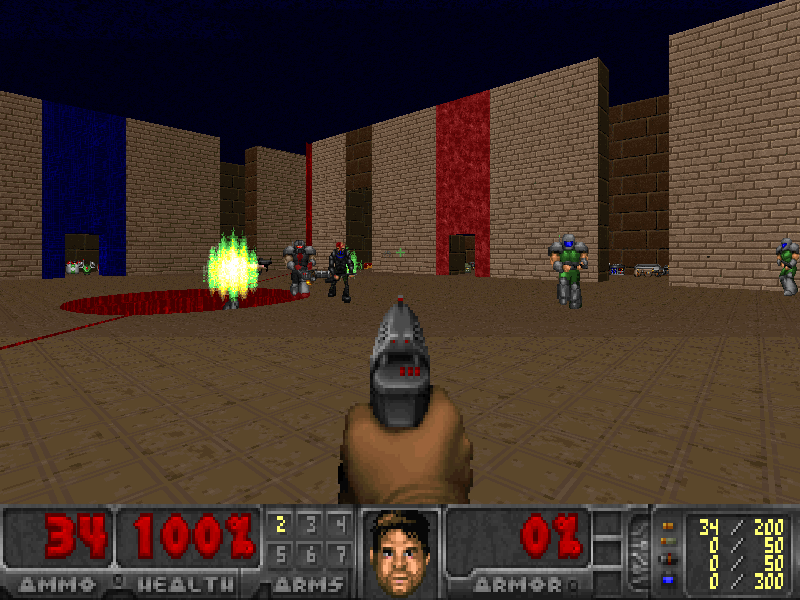
\includegraphics[width=\paperwidth,height=\paperheight,keepaspectratio=false]{img/arena.png}};
    \fill[night,opacity=0.78] (current page.south west) rectangle (current page.north east);
    \fill[night,opacity=0.9] (current page.south west) rectangle ([xshift=0.62\paperwidth]current page.north west);
  \end{tikzpicture}}
\begin{frame}[plain]
  \vspace*{10mm}
  {\color{accent}\small\bfseries\MakeUppercase{Uczenie ze wzmocnieniem}\par}
  \vspace{1.5mm}
  {\color{accent}\rule{18mm}{1.5pt}\par}
  \vspace{5mm}
  {\color{white}\fontsize{34}{38}\selectfont\bfseries Agent DQN w ViZDoom\par}
  \vspace{2mm}
  {\color{white!75!night}\Large Deathmatch -- postęp prac\par}
  \vspace{14mm}
  {\color{white!85!night}\normalsize Michał Piechota \quad\textbullet\quad Hubert Sobociński\par}
\end{frame}
}

% ============================================================
\renewcommand{\slidenum}{01}
\begin{frame}{Metoda: Double DQN z architekturą Dueling}
  \begin{columns}[T,onlytextwidth]
    \begin{column}{0.47\textwidth}
      {\footnotesize\textbf{Własna implementacja w PyTorch}: sieć, replay buffer,
      pętla uczenia i ewaluacji napisane od zera; trening na GPU Apple (MPS); 6,6\,mln parametrów.\par}
      \vspace{2mm}
      \begin{infocard}{\faBalanceScale}{Double DQN}
        Sieć online wybiera akcję, docelowa ją ocenia -- mniejsze przeszacowanie Q:\\[1mm]
        \raggedright
        $y = \sum_{k=0}^{2}\gamma^k r_{t+k}$\\
        $\quad+\,\gamma^3\,Q_{\bar\theta}\big(s_{t+3},\arg\max_{a'} Q_\theta(s_{t+3},a')\big)$\\[0.5mm]
        {\color{muted}cel 3-krokowy; strata Huber + BCE {\color{teal}głowicy pomocniczej}}
      \end{infocard}
      \begin{infocard}{\faCodeBranch}{Dueling}
        $Q(s,a) = V(s) + A(s,a) - \overline{A(s,\cdot)}$ -- wspólna wartość stanu, pomaga przy 31 akcjach.
      \end{infocard}
    \end{column}
    \begin{column}{0.49\textwidth}
      \centering
      \begin{tikzpicture}[
          box/.style={draw=faint,fill=card,rounded corners=1mm,minimum width=44mm,minimum height=6.5mm,font=\scriptsize,align=center},
          head/.style={draw=accent,fill=accentsoft,rounded corners=1mm,minimum width=20mm,minimum height=6.5mm,font=\scriptsize,align=center},
          arr/.style={-{Stealth[length=2mm]},muted,line width=0.8pt}]
        \node[box] (in) {wejście: 4 klatki RGB 60$\times$45 $\rightarrow$ 12$\times$45$\times$60};
        \node[box,below=2mm of in] (c1) {Conv 5$\times$5, 32, stride 2 + ReLU};
        \node[box,below=2mm of c1] (c2) {Conv 3$\times$3, 64, stride 2 + ReLU};
        \node[box,below=2mm of c2] (c3) {Conv 3$\times$3, 64, stride 1 + ReLU};
        \node[box,below=2mm of c3] (g) {$\oplus$ stan gry: 14 liczb $\rightarrow$ FC 64};
        \node[head,below left=3mm and -21mm of g] (v) {FC 512 $\rightarrow$ $V(s)$};
        \node[head,below right=3mm and -21mm of g] (a) {FC 512 $\rightarrow$ $A(s,\cdot)$};
        \node[box,below=10mm of g] (q) {$Q(s,\cdot)$: 31 wartości};
        \node[box,below=2mm of q,draw=teal] (aux) {wróg w kadrze? na celowniku?};
        \draw[arr] (in) -- (c1); \draw[arr] (c1) -- (c2); \draw[arr] (c2) -- (c3);
        \draw[arr] (c3) -- (g);
        \draw[arr] (g) -- (v); \draw[arr] (g) -- (a);
        \draw[arr] (v) -- (q); \draw[arr] (a) -- (q);
        \draw[arr,teal] (c3.east) -- ++(2.5mm,0) |- (aux.east);
      \end{tikzpicture}

    \end{column}
  \end{columns}
\end{frame}

% ============================================================
\renewcommand{\slidenum}{02}
\begin{frame}{Wejście i przestrzeń akcji}
  \begin{columns}[T,onlytextwidth]
    \begin{column}{0.4\textwidth}
      {\small\textbf{Wejście}\par}\vspace{1mm}
      \footnotesize
      \begin{itemize}\setlength\itemsep{1.5mm}
        \item RGB 320$\times$240 $\rightarrow$ \textbf{60$\times$45}, \textbf{stos 4 klatek}
          (12 kanałów) -- sieć widzi ruch potworów
        \item \textbf{Frame skip 4}: decyzja co 4.~tik
        \item Tak jak w literaturze: stos klatek dla sieci bez pamięci (DQN, Mnih 2015);
          Arnold i Sample Factory zamiast stosu używają LSTM
      \end{itemize}
      \vspace{1mm}
      \begin{infocard}{\faTachometer*}{Sprint -- zmierzone}
        \texttt{SPEED} podwaja ruch \textbf{i obrót}:
        14,1\textdegree{} $\rightarrow$ 28,1\textdegree{} na krok.
        Zwykły obrót = precyzyjne celowanie, sprint = szybkie szukanie celu.
      \end{infocard}
    \end{column}
    \begin{column}{0.56\textwidth}
      {\small\textbf{31 akcji} \scriptsize\color{muted}(wcześniej 18: jeden przycisk naraz, 10 martwych/zbędnych)\par}
      \vspace{1mm}
      \scriptsize
      \renewcommand{\arraystretch}{1.2}
      \begin{tabular}{@{}>{\color{accent}\bfseries}l>{\raggedright\arraybackslash}p{0.72\linewidth}@{}}
        \toprule
        podstawowe (8) & brak akcji, strzał, przód, tył, w lewo, w prawo, obrót L/P \\
        broń (2) & następna / poprzednia broń \\
        strzał + ruch (6) & obrót L/P, przód, tył, w lewo, w prawo -- ze strzałem \\
        ruch (4) & przód + obrót L/P, \emph{circle strafe} L/P \\
        sprint (6) & sprint + przód / tył / lewo / prawo / obrót L/P \\
        sprint-trójki (5) & sprint + przód + obrót L/P, sprint + przód / lewo / prawo + strzał \\
        \bottomrule
      \end{tabular}

      \vspace{2mm}
      {\scriptsize\color{muted}Agent może strzelać w ruchu i w trakcie obrotu.
      Usunięte: \texttt{STRAFE} (dubluje ruch boczny) i wybór broni po numerze.\par}
    \end{column}
  \end{columns}
\end{frame}

% ============================================================
\renewcommand{\slidenum}{03}
\begin{frame}{Kształtowanie nagrody}
  \begin{columns}[T,onlytextwidth]
    \begin{column}{0.5\textwidth}
      \scriptsize
      \renewcommand{\arraystretch}{1.3}
      \begin{tabular}{@{}>{\raggedright\arraybackslash}p{0.6\linewidth}>{\raggedleft\arraybackslash}p{0.34\linewidth}@{}}
        \toprule
        \textbf{Składnik} {\color{muted}(różnice zmiennych gry)} & \textbf{Waga} \\
        \midrule
        zabójstwo \textbf{po własnym trafieniu} & nagroda z gry \\
        zadane obrażenia & $+0{,}05$ / pkt \\
        trafienie (\texttt{HITCOUNT}) & $+0{,}1$ \\
        utrata zdrowia & $-0{,}01$ / HP \\
        strzał bez trafienia & $-0{,}01$ \\
        leczenie & $+0{,}02$ / HP \\
        amunicja, gdy pula $<10\%$ & $+0{,}1$ / podniesienie \\
        pancerz & $+0{,}01$ / pkt \\
        przebyta droga & $+0{,}0005$ / jedn. \\
        śmierć & $-1$ \\
        \midrule
        suma skalowana & $\times\,0{,}1$ \\
        \bottomrule
      \end{tabular}
    \end{column}
    \begin{column}{0.46\textwidth}
      \begin{infocard}{\faExclamationTriangle}{Atrybucja zabójstw}
        Tylko \textbf{15 ze 159} (9\%) zabójstw agenta losowego nastąpiło
        w~ciągu 2\,s od jego trafienia -- reszta to walki między potworami.
        Za zabójstwo płacimy tylko, gdy \texttt{HITCOUNT} wzrósł w ostatnich 70 tikach.
      \end{infocard}
      \begin{infocard}{\faArrowUp}{Względem planu ze slajdów}
        Trafienie liczone obrażeniami; apteczka proporcjonalna do odzyskanego HP;
        dodane: pancerz, droga, skalowanie. Amunicja tylko przy pustej puli --
        $+0{,}05$/sztukę agent \textbf{farmił} (przedmioty się odradzają).
      \end{infocard}
      {\scriptsize\color{muted}\faInfoCircle\hspace{1.5mm}Ewaluacja zawsze na oryginalnej
      nagrodzie gry i~metrykach z~protokołu.\par}
    \end{column}
  \end{columns}
\end{frame}

% ============================================================
\renewcommand{\slidenum}{04}
\begin{frame}{Hiperparametry i przebieg treningu}
  \begin{columns}[T,onlytextwidth]
    \begin{column}{0.47\textwidth}
      \footnotesize
      \renewcommand{\arraystretch}{1.2}
      \begin{tabular}{@{}>{\raggedright\arraybackslash}p{0.5\linewidth}>{\raggedleft\arraybackslash}p{0.44\linewidth}@{}}
        \toprule
        \textbf{Parametr} & \textbf{Wartość} \\
        \midrule
        budżet & 10\,mln klatek gry \\
        dyskonto $\gamma$ & 0,99 \\
        cel TD & 3-krokowy \\
        optymalizator, lr & Adam, $5\!\cdot\!10^{-5} \rightarrow 10^{-5}$ \\
        batch & 64 \\
        replay buffer & 400\,tys. przejść \\
        start uczenia & po 20\,tys. kroków \\
        aktualizacja sieci & co 4 kroki \\
        kopia sieci docelowej & co 10\,tys. kroków \\
        $\varepsilon$ & $1 \rightarrow 0{,}05$ przez 25\% treningu \\
        $\varepsilon$ w ewaluacji & 0,05 \\
        przycinanie gradientu & 10 \\
        \bottomrule
      \end{tabular}
    \end{column}
    \begin{column}{0.49\textwidth}
      \begin{infocard}{\faMemory}{Replay buffer na klatkach}
        Każda klatka zapisana raz (uint8); stosy składane przy losowaniu,
        bez przekraczania granicy epizodu $\Rightarrow$ 3,2\,GB zamiast $\sim$26\,GB.
      \end{infocard}
      \begin{infocard}{\faChartLine}{Ewaluacja w trakcie treningu}
        Co 100\,tys. klatek: 10 epizodów na stałym seedzie silnika,
        $\varepsilon=0{,}05$ $\rightarrow$ krzywe uczenia. Najlepszy checkpoint
        wg zabójstw przypisanych agentowi.
      \end{infocard}
      \begin{infocard}{\faStopwatch}{Koszt}
        \textasciitilde165 kroków/s na Apple M5 (MPS);
        wąskim gardłem jest krok uczenia sieci (15\,ms).
        Logi: TensorBoard + CSV.
      \end{infocard}
    \end{column}
  \end{columns}
\end{frame}

%%RESULTS%%

\end{document}
